\documentclass{beamer}

\usepackage{graphicx,hyperref,url}

\usepackage[T1]{fontenc}    %%% UNICODES etc
\usepackage[utf8]{inputenc}

\usepackage{booktabs}
\usepackage[brazil]{babel}
\usepackage{lmodern, comment}
\usepackage{amsmath,amssymb,amstext}
\usepackage{xcolor}
\usepackage{pifont}
%%%\usepackage{fontspec}
\usepackage{marvosym}

%%% TO DISCOVER ERRORS 
%\DeclareUnicodeCharacter{00B4}{\ensuremath{\theta}}

%% FOR ASP
\usepackage{listings}
\lstset{basicstyle=\ttfamily,escapechar=\%,escapeinside={\#(}{\#)}}


%%% FIGS \graphicspath{{figures/}{../figures/}{C:/Users/me/Documents/project/figures/}}

\graphicspath{ {figures/} {../ia_combinatoria/figures/} }
%%%%\graphicspath{ {/home/user} }
\definecolor{azulclaro}{rgb}{0.9,0.9,0.9}
\definecolor{mygreen}{rgb}{0,0.6,0}
\definecolor{mygray}{rgb}{0.5,0.5,0.5}
\definecolor{mymauve}{rgb}{0.58,0,0.82}
\definecolor{darkgray}{rgb}{.4,.4,.4}
\definecolor{purple}{rgb}{0.65, 0.12, 0.82}


\lstset{ 
  %  label={pgm_ex01},
    backgroundcolor=\color{azulclaro}, 
    language=Haskell, %%Miranda,%%Perl,%%%Python, %%Mercury,
    showstringspaces=false,
    basicstyle=\bf\scriptsize\ttfamily,
%%      basicstyle= \footnotesize %%% TESTAR
%%      keywordstyle=\bfseries\color{green!40!black},
    keywordstyle=\textbf{\color{mygreen}}, 
    otherkeywords={*, \%, array, constraint, solve, output,  show, "/\", satisfy, set, of, if, then, elseif, float, search},
%%  keywordstyle=\color{blue},       % keyword style
%%    commentstyle=\itshape\color{purple!40!black},
      commentstyle=\color{orange},    % comment style
      identifierstyle=\color{blue},
      stringstyle=\color{orange},
      stringstyle=\color{mymauve},
      numbers=left,  % where to put the line-numbers; possible values are (none, left, right)
      numbersep=5pt,   % how far the line-numbers are from the code
      numberstyle=\tiny\color{magenta},
      keepspaces=true      
    % %caption={LEGENDA no source PASCAL ficou OK},
}



\title[Combinatorial  Optimization] % (optional, use only with long paper titlebg=blue!20!white,s)
{Map Coloring Problem with \\ \textit{Answer Set Programming -- clingo}\\ An Encoding}
%\subtitle
%{About some things}
\author[Claudio Cesar de Sá] % (optional, use only with lots of authors)
{Claudio Cesar de Sá}%\inst{1}
% - Give the names in the same order as the appear in the paper.
% - Use the \inst{?} command only if the authors have different
%   affiliation.

\institute[WhatsTV]{Independent Researcher}

% - Use the \inst command only if there are several affiliations.
% - Keep it simple, no one is interested in your street address.

\date[\today] % (optional, should be abbreviation of conference name)


\begin{document}

\begin{frame}
  \titlepage
  
\end{frame}



% Structuring a talk is a difficult task and the following structure
% may not be suitable. Here are some rules that apply for this
% solution: 

% - Exactly two or three sections (other than the summary).
% - At *most* three subsections per section.
% - Talk about 30s to 2min per frame. So there should be between about
%   15 and 30 frames, all told.

% - A conference audience is likely to know very little of what you
%   are going to talk about. So *simplify*!
% - In a 20min talk, getting the main ideas across is hard
%   enough. Leave out details, even if it means being less precise than
%   you think necessary.
% - If you omit details that are vital to the proof/implementation,
%   just say so once. Everybody will be happy with that.

%%%%%%%%%%%%%%%%%%%%%%%%%%%%%%%%%%%%%%%%%%%%%%%%%%%%%%%


\begin{frame}

\begin{block}{Road map of this presentation:}
%  \tableofcontents

\begin{enumerate}

  \item  About the  ASP (clingo)
  \item  Requisites
  \item  The problem: map coloring
  \item  Discussion of this (NP-complete) problem
  \item  A modelling in ASP
  \item  A solution in clingo
  \item  Conclusions

  \end{enumerate}

\end{block}

\pause
\textbf{\textcolor{red}{Attention: some background in logic and declarative language is recommended!}}


\end{frame}


%%%%%%%%%%%%%%%%%%%%%%%%%%%%%%%%%%%%%%%%%%%%%%%%%%%%%%%
\begin{comment}
\section{Para efeitos de TEMPLATE}
\begin{frame}
\frametitle{Nome do SLIDE}
\begin{block}{Nome do Bloco}
  \begin{itemize}
   \item T1

    \item<2-> T2

    \item<3-> T3

  \item<4-> 

    \item<5-> 
    
        \item<6-> 
    \end{itemize}
  
\end{block}

\end{frame}
\end{comment}
%%%%%%%%%%%%%%%%%%%%%%%%%%%%%%%%%%%%%%%%%%%%%%%%%%%%%%%




%%%%%%%%%%%%%%%%%%%%%%%%%%%%%%%%%%%%%%%%%%%%%%%%%%%%%%%%%
\section{Nutshell}
\begin{frame}{Answer Set Programming\\[-2pt]{\small\emph{in a Nutshell}  (this page was borrowed from official repository):} }
  \begin{itemize}
  \item <2->
    ASP is an approach to \alert{declarative problem solving},   combining
    \begin{itemize}
    \item a rich yet simple modeling language
    \item with high-performance solving capacities
    \end{itemize}
    % tailored to Knowledge Representation and Reasoning % (KRR)
  \item <3-> ASP has its roots in
    \begin{itemize}
    \item (deductive) databases
    \item logic programming (with negation)
    \item (logic-based) knowledge representation and (non-monotonic) reasoning
    \item constraint solving (in particular, SATisfatibility testing)
    \end{itemize}
  \item <4-6>
    ASP allows for solving all search problems in $NP$ (and $NP^{NP}$)
    \\in a uniform way % (being more compact than SAT)
  \item <5-6>
    ASP fundaments in: propositional, first-order, auto-epistemic, default. Many aspects in theory and programs.
  \item <6-6> ASP embraces many emerging application areas
  \end{itemize}
\end{frame}


\begin{frame}%[allowframebreaks]

\frametitle{Historic and references:}

\begin{block}{}
  \begin{itemize}
   \item This programming language has its origin at the University of Potsdam (Universität Potsdam) -- 1999
   
   \item  \textbf{Potassco}, the \textbf{Po}tsdam \textbf{A}nswer \textbf{S}et \textbf{S}olving \textbf{Co}llection -- \url{https://potassco.org/}
   
   \item Official repository with a full-course: \url{https://github.com/potassco-asp-course/}

  \item Support to start: an active forum and a course covered by videos in the Youtube
  
  \item \textcolor{red}{This presentation and its code}:\\
   \textbf{\textcolor{blue}{\url{https://github.com/claudiosa/CCS/tree/master/asp_Answer_Set_Programming}}}
  
  \item Books: 

 \end{itemize}
  
\end{block}

\end{frame}


%%% capa dos livros


\begin{frame}
	\frametitle{Some References:}
	
\begin{figure}[tbp]
  \centering
	 
\includegraphics[width=0.4\textwidth , height=0.55\textheight]{cover_book_vladmir.jpg}
	 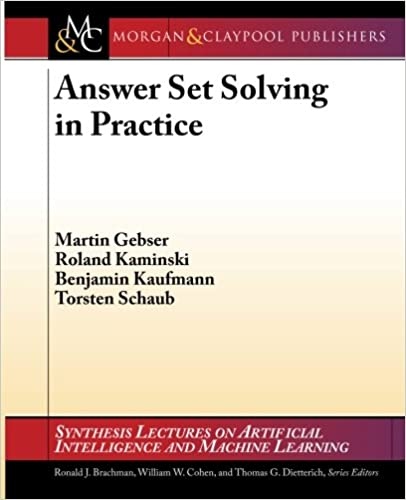
\includegraphics[width=0.4\textwidth , height=0.55\textheight]{cover_book_roland.jpg}
  %\caption{Estou usando o do Vladmir}
	
	\end{figure}
\end{frame}

%%%%%%%%%%%%%%%%%%%%%%%%%%%%%%


\begin{frame}[fragile]
\frametitle{Characteristics:}
\begin{block}{}
  \begin{itemize}
  
  
  \item The theoretical background has the roots  from many logics: propositional, first-order, circumscription (world closed supposition), default and the negation as a fail.
  
  \item The concept of  \textbf{stable model} to deduce one or more answers.

  \item The combinatorial problems are well modelled with ASP (\textit{wear as glove}) 

  \item The enconding declare \textbf{decisions} e \textbf{constraints}

  %    \item Tudo isto na ordem de milhões!
      
    %  \item Na indústria: desde gerenciador de pacotes do Debian a sistemas da NASA
        

    \end{itemize}
  
\end{block}

\end{frame}

\begin{comment}
xxxxxxxxxxxxxxxxxxxxxxxxxxxxx COMMENTED
\end{comment}

% ----------------------------------------------------------------------
\begin{frame}[c]{Modelling, grounding and resolution:}
%\frametitle{Resumindo ...}
\begin{center}
	\small
   \setlength{\unitlength}{.7pt}
   \begin{picture}(420,200)(-210,-35)
   	   \put(-200,110){\framebox(80,40){Problem}}
	   \put(-200,-20){\framebox(80,40){\shortstack{Logic\\Program}}}
    	\put(-80,-15){\framebox(60,30){Grounder}}
		\put(  20,-15){\framebox(60,30){Solver}}
		\put( 120,-20){\framebox(80,40){\shortstack{Stable\\Models}}}
		\put( 120,110){\framebox(80,40){Solution}}
		\put(-120,0){\vector(1,0){40}}
		\put( -20,0){\vector(1,0){40}}
		\put(  80,0){\vector(1,0){40}}
		\put(-160,110){\vector(0,-1){90}}
		\put( 160, 20){\vector(0, 1){90}}
		\put(-217, 62.5){\emph{Modeling}}
		\put( 165, 62.5){\emph{Interpreting}}
		\put( 0,-32.5){\makebox(0,0){\emph{Solving}}}
   \end{picture}
  %\end{center}
  \end{center}
Source: \url{https://github.com/potassco-asp-course/}
\end{frame}

%%%%%%%%%%%%%%%%%%%%%%%%%%%%%%%%%%%%%%%%%%%%%%%%%%%%%%\

\section{Definitions -- Graph coloring:}
\begin{frame}[fragile] 
	%\frametitle{Graph coloring -- a set of problems related}
	\frametitle{A case-study: Map Coloring Problem (a practical problem from graph coloring)}
		
	
\begin{figure}[tbp]
  \centering
%	 
\includegraphics[width=0.4\textwidth , height=0.55\textheight]{cover_book_vladmir.jpg}
	 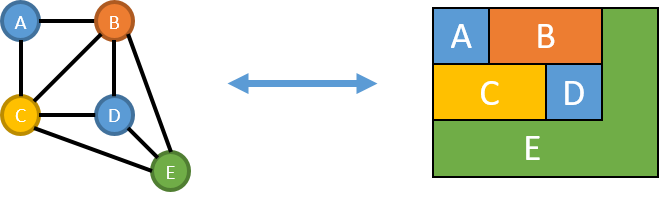
\includegraphics[width=0.9\textwidth , height=0.3\textheight] {graph_coloring_equivalence.png}
  \caption{Let's consider a planar map for readgibility}
	
	\end{figure}
{\small	
\begin{block}{}
  \begin{itemize}
 % \setlength\itemsep{4pt}
  \item Input: a graph (map) $G$ with $n$ vertices (countries) and  integer $k$ (colors)
  \item Output: does $G$ admit a proper vertex coloring with k colors?
  \item Complexity:	NP-Complete
  \item Optimization: NP-Hard (lesser chromatic number -- $k$)
     \end{itemize}
 \end{block}
}

\end{frame}



\begin{frame}[fragile] 

	\frametitle{Borrowed and adapted from:\\ {\small \url{https://github.com/potassco-asp-course/modeling/}}} 
 
 \begin{itemize}
  \item \structure{Problem instance:} \ A map consisting of countries and neighborhood  (frontiers)
    \begin{itemize}
    \item facts formed by predicates \texttt{country/1} and \texttt{neighbour/2}
    \item  facts formed by predicate  \texttt{color/1}
    \end{itemize}
    \medskip
  \item \structure{Problem class:} \ Assign each country one color such that no two countries connected
    or  neighbour  have the same color
    \medskip
  \item In other words,
    \begin{enumerate}
    \item Each country has one color
    \item Two connected (neighbour) countries must not have the same color
    \end{enumerate}
  \end{itemize}
\end{frame}

%%%%%%%%%%%%%%%%%%%%%%%
\begin{frame}[fragile] 

\frametitle{Let's paint this map with \(\textbf{k}\) colors:}
	
\begin{figure}[tbp]
  \centering
% 
\includegraphics[width=0.4\textwidth , height=0.55\textheight]{cover_book_vladmir.jpg}
    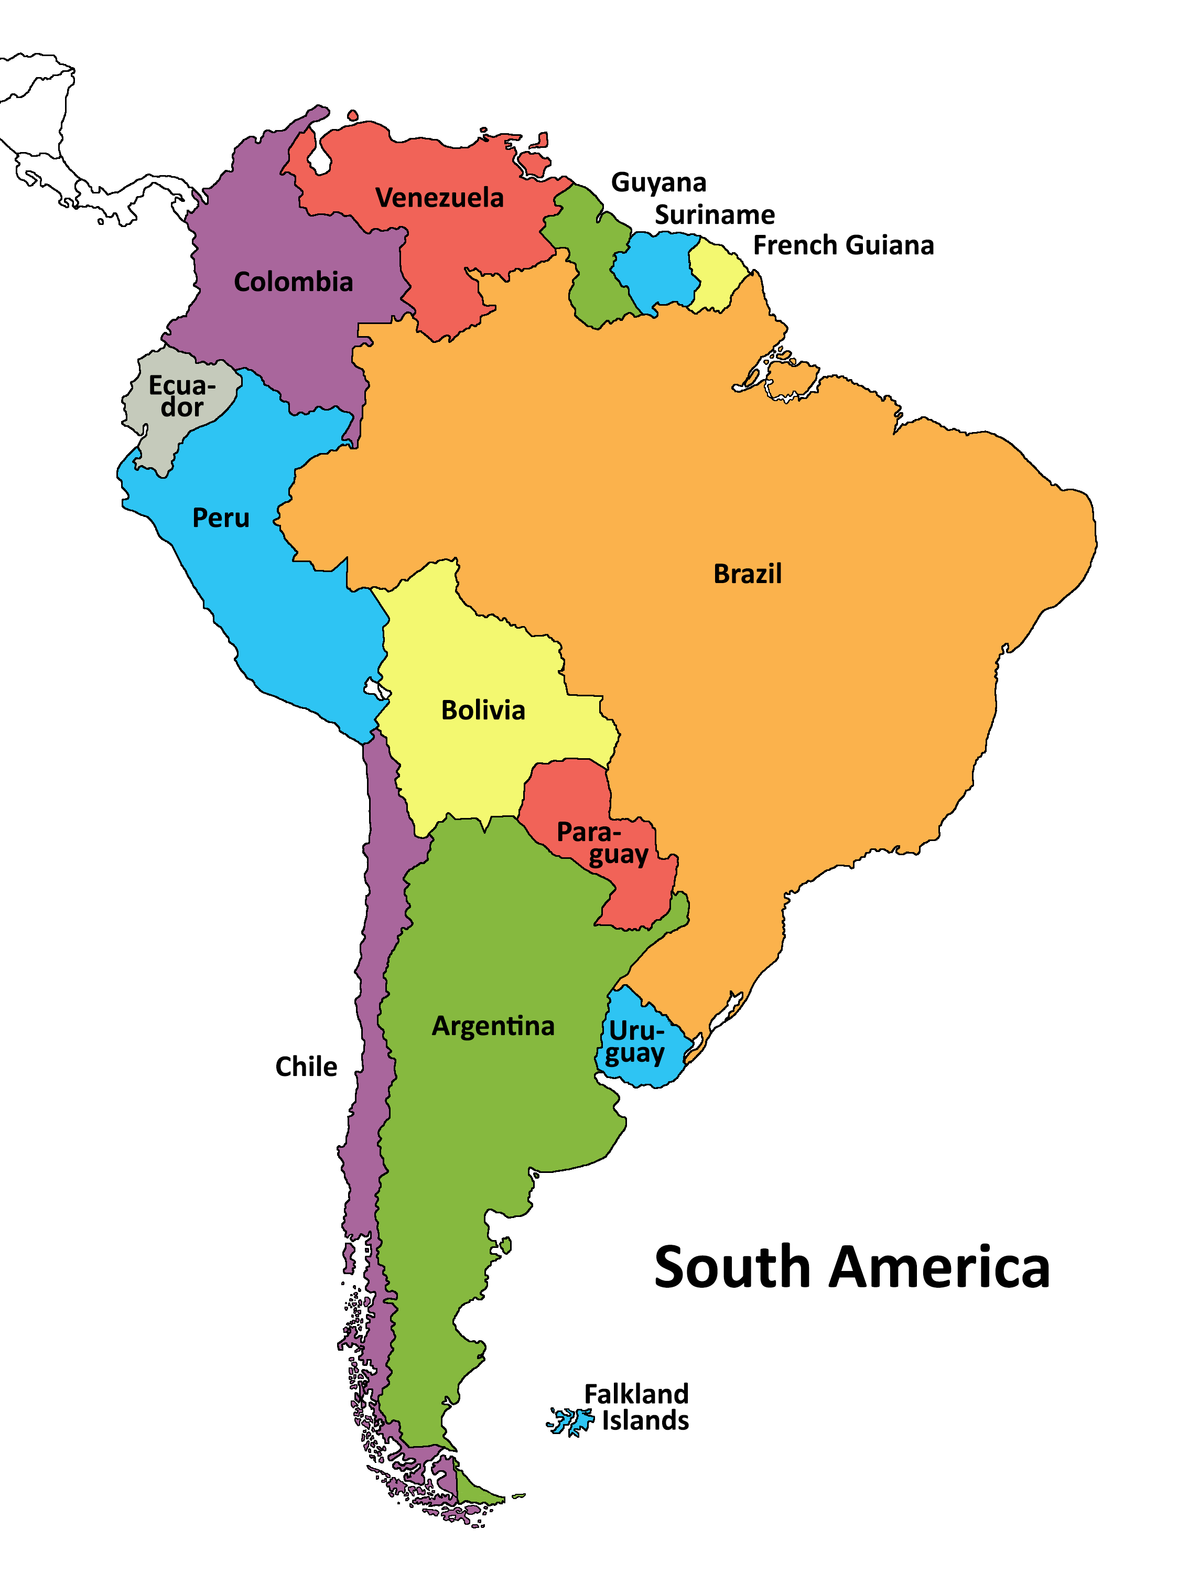
\includegraphics[width=0.6\textwidth , height=0.65\textheight] {south_america.png}
   \caption{South America map, the author had the input data --  \Smiley{}}
	
\end{figure}
	
\pause
Finally, let's try to  find a minimal color number to paint this map, without any neighbour country have the same color!

\end{frame}


%%%%%%%%%%%%%%%%%%%%%%%%%%%%%%%%%%%%%%%%%%%%%%%%%%%%%%%
\section{Modelling}
\begin{frame}[fragile] 
	\frametitle{Some comments:}
	
\begin{block}{}
  \begin{itemize}
  % \setlength\itemsep{4pt}
 \item Theoretical details can be found in: \url{https://en.wikipedia.org/wiki/Graph_coloring}

 \item The modelling was almost immediate with an old Prolog code from the author:
\url{https://github.com/claudiosa/CCS/......}

  \item Many approaches for this problem can be taken: Simulated Annealing, Ant Colony, Depth-First Search, ..., meta-heuristics in general presents a good efficiency
  \item The full code discussed here is found in:\\ \url{https://github.com/claudiosa/CCS/tree/master/asp_Answer_Set_Programming/map_coloring.lp}
  \item We are commenting it in parts

   \end{itemize}
 \end{block}
	
	
%\textcolor{red}{xxxxxxxxxxxxxxxxxxxxxxxxxxx!}	
\end{frame}
%%%%%%%%%%%%%%%%%%%%%%%%%%%%%%%%%%%%%%%%%%%%%%%%%%%%%%%
\begin{frame}[fragile] 
\frametitle{Colors available (k) and countries (n):}
	
{\small
\begin{verbatim}
%% Colors
color(red).
color(blue).
color(green).
color(yellow).
%% Countries
country(antilles).       country(argentina).
country(bolivia).        country(brazil).
country(columbia).       country(chile).
country(ecuador).        country(french_guiana).
country(guyana).         country(paraguay).
country(peru).           country(surinam).
country(uruguay).        country(venezuela).

\end{verbatim}
}	
\textcolor{red}{Ground terms, exactly written like Prolog syntax.}
\end{frame}


%%%%%%%%%%%%%%%%%%%%%%%%%%%%%%%%%%%%%%%%%%%%%%%%%%%%%%%

\begin{frame}[fragile] 
	\frametitle{The map, countries and their relations with neighbours:}
	
{\small
\begin{verbatim}
neighbour(antilles,venezuela).   neighbour(argentina,bolivia).
neighbour(argentina,brazil).     neighbour(argentina,chile).
neighbour(argentina,paraguay).   neighbour(argentina,uruguay).
neighbour(bolivia,brazil).       neighbour(bolivia,chile).
neighbour(bolivia,paraguay).     neighbour(bolivia,peru).
neighbour(brazil,columbia).      neighbour(brazil,french_guiana).
neighbour(brazil,guyana).        neighbour(brazil,paraguay).
neighbour(brazil,peru).          neighbour(brazil,surinam).
neighbour(brazil,uruguay).       neighbour(brazil,venezuela).
neighbour(chile,peru).           neighbour(columbia,ecuador).
% To avoid duplication of the facts above
neighbour(X,Y) :- neighbour(Y,X). 
% To obtain more symmetric results at the end
\end{verbatim}
}	
\textcolor{red}{Another representation is possible, but until now, everything was reused -- kept simple as possible!}
\end{frame}


%%%%%%%%%%%%%%%%%%%%%%%%%%%%%%%%%%%%%%%%%%%%%%%%%%%%%%%
\begin{frame}[fragile] 
	\frametitle{Modelling the problem under its requisites:}
	
{\small
\begin{verbatim}
%%  Country X Colors - Assign any color for each country
1 { country_color(P, C) : color(C) } 1 :- country(P).

%% Brazil must be green
:- not country_color(brazil,green).
%% OR
%% country_color(brazil,green).

%% Finally: none adjacent countries receive at the same color
% C != C1 :- country_color(P, C), country_color(P1, C1), 
             neighbour(P,P1).
%% OR -- by Susana - ASP Community         
:- country_color(P, C), country_color(P1, C), neighbour(P,P1).
\end{verbatim}
}	
\textcolor{red}{Basically, that's all!}
\end{frame}


%%%%%%%%%%%%%%%%%%%%%%%%%%%%%%%%%%%%%%%%%%%%%%%%%%%%%%%%%%%%%%%%%%%%%%%%%%%%%%%%%%%%%%%%%%%%%%

\begin{frame}[fragile]
	\frametitle{Preparing for a optimization:}

{\small
\begin{verbatim}
	
%% number of colors used
n_colors(N) :-   N = #count{C : country_color(P,C)}.

%% A minimization on this value
#minimize{ N : n_colors(N) }.

%% OUTPUT
#show country_color/2.
#show n_colors/1.
\end{verbatim}
}	
\textcolor{red}{\hrule \vskip 0.2cm That's all!}
\end{frame}
%%%%%%%%%%%%%%%%%%%%%%%%%%%%%%%%%%%%%%%%%%%%%%%%%%%%%%%
%\begin{frame}[allowframebreaks]
\begin{frame} [fragile]
\frametitle{An output:}
	
{\small
\begin{verbatim}
clingo ../map_coloring.lp 0 --out-ifs='\n' --out-atomf=%s. 
clingo version 5.3.0
Reading from ../map_coloring.lp
Solving...
Answer: 1
country_color(argentina,red).
country_color(columbia,red).
country_color(surinam,red).
country_color(guyana,blue).
country_color(paraguay,blue).
...........................
country_color(french_guiana,yellow).
country_color(venezuela,yellow).
n_colors(4).
Optimization: 4
OPTIMUM FOUND
Models       : 1
  Optimum    : yes
Optimization : 4
Calls        : 1
Time         : 0.003s (Solving: 0.00s 1st Model: 0.00s Unsat: 0.00s)
CPU Time     : 0.003s
\end{verbatim}
}	
\end{frame}


%%%%%%%%%%%%%%%%%%%%%%%%%%%%%%%%%%%%%%%%%%%%%%%%%%%%%%%

\begin{frame}[fragile] 
 \frametitle{For future explorations:}

A cool suggestion from Adam Smith:  \emph{express preferences for country colors at a lower priority, searching for a min colors number. In the sequence, try to find the max number with the countries satisfy with their preferences. Here's a little snippet that shows mixing minimization and maximization at different priorities}:

{\small
\begin{verbatim}
% minimize number of colors used at higher priority
color_used(C) :- country_color(P,C).
#minimize {1,C@2:color_used(C)}. 

% maximize number of color preferences satisfied at lower priority
color_preference(brazil,green).
preference_satisfied(P) :- color_preference(P,C), 
                           country_color(P,C)
#maximize {1,P@1:preference_satisfied(P,C) }.	
\end{verbatim}
}	

\textcolor{red}{Not tested yet, but, surely it works!}

\end{frame}


%%%%%%%%%%%%%%%%%%%%%%%%%%%%%%%%%%%%%%%%%%%%%%%%%%%%%%%

\begin{frame}[fragile] 
	\frametitle{Conclusions:}
	
\begin{block}{}
\begin{itemize}
  

  \item ASP is strongly declarative (roots from the logic to attack the problems representation)
  
  \item Generate and test methodology
    
  \item ASP's workflow, modeling, grounding, solving
    (and optimizing)
    %\smallskip
  \item clingo = gringo$+$clasp $+$ \dots

  \item Allows you to embed a Python coding in order to minimize the difficulties (\Frowny) of input and output data
		
   \item An encoding in ASP is excellent exercise to keep your mind very active!

	\item Finally, a huge gratitude for the \textbf{potassco-users list}, always reactive for my silly doubts,  where I had been learning much.
		
	\end{itemize}
\end{block}
\end{frame}



%%%%%%%%%%%%%%%%%%%%%%%%%%%%%%%%%%%%%%%%%%%%%%%%%%%%
\section*{Contact}

\begin{frame}
\frametitle{Contact and Comments (are must welcome\ \Smiley):}
  
\begin{block}{}
  % Keep the summary *very short*.
  \begin{itemize}
  \item \url{https://claudiocesar.wordpress.com/}
%   \item \url{https://github.com/claudiosa}
   \item \textcolor{red}{This presentation and the code discussed}:\\
   \textbf{\textcolor{blue}{\url{https://github.com/claudiosa/CCS/tree/master/asp_Answer_Set_Programming}}}
   \item There is a directory to Youtube!
    
   %\item In this  git, repository CCS $\Rightarrow$ asp...
   %%\item Email: \url{claudio.sa@udesc.br}
  \item \Letter: \url{ccs1664@gmail.com}
  \item This material has a partial support from WhatsTV Inc. \url{https://en.whatstv.com.br/}, here our gratitude!
  \item \textit{Thank you so much}!

  \end{itemize}
  \end{block}

\end{frame}


%%%%%%%%%%%%%%%%%%%%%%%%%%%%%%%%%%%%%%%%%%%%%%%%%%%%%%%
\end{document}